\chapter{Modelo para las interacciones de aumentación}

\label{cha:interacciones}

\chaptermark{Interacciones de aumentación}

Las interacciones de aumentación constituyen la parte dinámica de la aplicación WebMakeUp. Las interacciones se realizan entre el usuario y los widgets. El usuario, a medida que va trabajando con el sitio web, puede generar diferentes tipos de eventos Javascript (clic-ar, pasar el ratón por encima, escribir en un widget, arrastrar y soltarlo, etc.).

En una aumentación web, además de añadir y quitar contenido de un sitio web, se le puede dotar de interacción usuario-widgets, haciéndolo más dinámico. Por ejemplo, puede existir un botón que al pulsarlo muestre u oculte cierto contenido, o que al escribir en un cuadro de texto si la palabra está mal formada se muestre otro widget en color rojo indicando que hay un error. Todo esto y mucho más se hace mediante Javascript, que es el encargado en el lado cliente de todo el dinamismo.

El problema surge cuando un usuario para realizar una aumentación tiene que aprender a programar la escucha de estos eventos (para saber cuándo se producen). Pero no solo eso, sino que también las funciones que se tienen que realizar cuándo este evento se produce (concepto conocido como manejador o handler).

Por tanto, en WebMakeUp surge la necesidad de tener un modelo de interacciones de aumentación que se encargue de gestionar todo este proceso. Esto evitará que el usuario, por un lado, tenga que aprender Javascript, y por otro lado, disponer de una cantidad de tiempo considerable para desarrollar la aumentación.

Pero antes de ello, es necesario saber cómo se va a estructurar el editor WebMakeUp. De esta idea surge la primera tarea de WebMakeUp, estudiar diferentes herramientas de edición existentes en el mercado (Apartado \ref{sec:editoresRetoque}). Así se puede representar, por una parte, el trabajo de los widgets (línea de investigación que no se ha realizado en este PFG), y por otra, representar las interacciones entre widgets (que se ha realizado en gran medida en este PFG y es en la que se centrará este capítulo).

Para la representación del modelo de interacciones, se propuso realizarlo en base a diagramas de transición de estados (que se explicará en el Apartado \ref{sec:modeloSTD}). Aunque, tras pruebas con usuarios finales de la aplicación, se decide desechar la idea y sustituirla por otra más sencilla basada en blinks (que se explica en el Apartado \ref{sec:modeloBlinks}).

\section{Editores de retoque}
\label{sec:editoresRetoque}

El estudio de editores de retoque tiene diferentes finalidades:
\begin{itemize}
\item{Permite conocer las herramientas que están presentes en el mercado y que utilizan usuarios finales habitualmente. Esto puede ayudar a encontrar un equilibrio entre el lenguaje de programación y el lenguaje que conoce el usuario final.}
\item{Buscar cómo se representan algunos aspectos técnicos y complejos para un usuario final. Ya sea utilización de iconos, el entorno de trabajo al que está habituado el usuario final, etc.}
\item{Buscar si existen herramientas similares a lo que con WebMakeUp se tenía intención de hacer.}
\item{Descartar ideas complejas, centrándose en diseñar un DSL (lenguaje específico de dominio) sencillo para un usuario, donde el objetivo es que prácticamente cualquier usuario de sitios webs pueda diseñar una aumentación.}
\end{itemize}

Para marcar un primer objetivo, hay que buscar información general sobre diferentes editores de uso común. Para ello hay que basarse en editores donde el propósito era igual que el de WebMakeUp, trabajar sobre un artefacto ya existente y crear un mod a partir de él. Para ello se tiene que buscar herramientas en las que basar la metáfora, con tal de poder decir \emph{si sabes utilizar X herramienta, sabes utilizar WebMakeUp}.

En el cuadro \ref{tab:EditoresRetoque} se muestran algunos de los editores que se estudiaron donde las principales características a valorar eran la relación que se pudiera asociar entre la interfaz del editor y las necesidades de mostrar widgets e interacciones entre ellos que tenía WebMakeUp.

\begin{table}
\begin{center}
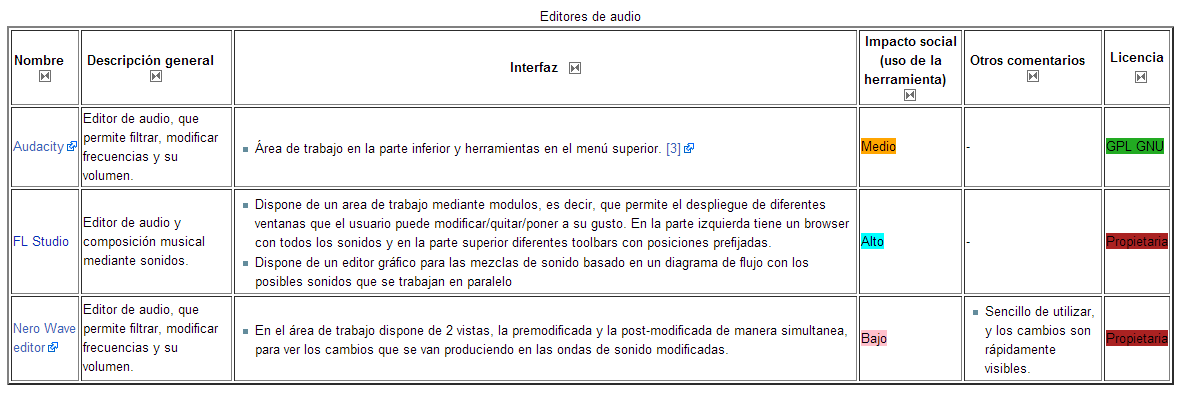
\includegraphics[width=0.95\textwidth]{figs/4-EditoresDeAudio.png}
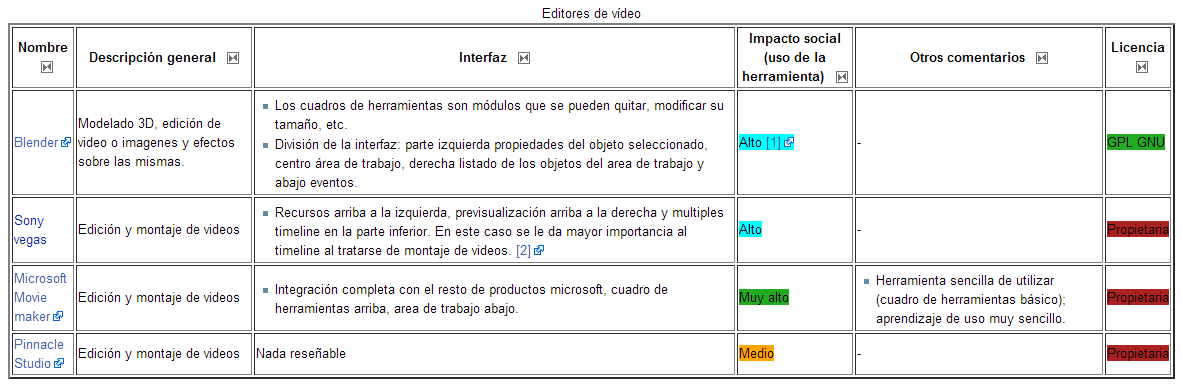
\includegraphics[width=0.95\textwidth]{figs/4-EditoresDeVideo.png}
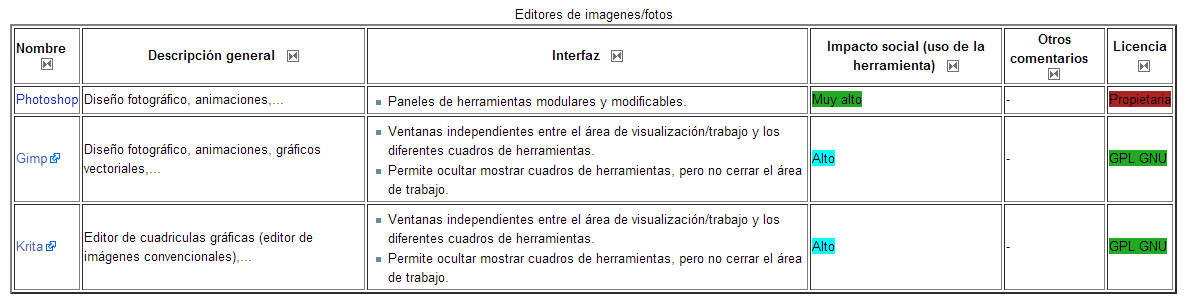
\includegraphics[width=0.95\textwidth]{figs/4-EditoresDeImagenes.png}
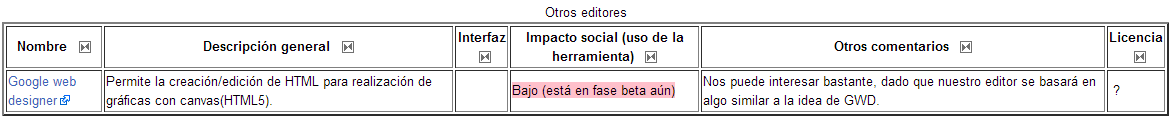
\includegraphics[width=0.95\textwidth]{figs/4-EditoresDeOtroTipo.png}
\caption{Estudio de editores de retoque de uso general (audio, vídeo, imágenes y web).}
\label{tab:EditoresRetoque}
\end{center}
\end{table}

Tras realizar un pequeño estudio general se decide tomar como referencia Photoshop, por varias razones:
\begin{itemize}
\item{Es una de las aplicaciones de edición más conocidas y usadas del mercado.}
\item{El entorno de trabajo es cómodo para el usuario, abre el editor, escoge una imagen, se muestra en el lienzo y a partir de ahí trabaja prácticamente usando sólo el lienzo. En WebMakeUp también se puede realizar eso, abrir el sitio web y a partir de ahí trabajar sobre el Canvas del sitio web de manera gráfica. En la Figura \ref{fig:IDEPhotoshop} de color rojo se refleja el Canvas de Photoshop. Esto se complementa con el artículo \cite{WebSpec}, que recomienda el uso de lenguajes gráficos para la interacción y navegación.}
\item{Disponía de una característica similar a las interacciones. En Photoshop existe una línea temporal para las animaciones, donde a medida que transcurre el tiempo puede ir variando la imagen. En la Figura \ref{fig:IDEPhotoshop} de color verde, se refleja la línea temporal de la animación en Photoshop. En WebMakeUp no existe una línea temporal, pero sí que va variando el contenido y el comportamiento de los widgets del sitio web a medida que el usuario interacciona con él.}
\item{En el lateral izquierdo existen herramientas para la edición de imágenes en Photoshop. En WebMakeUp ese panel puede ser útil para tener herramientas relacionadas con widgets, como por ejemplo un repositorio de widgets.}
\end{itemize}

\begin{figure}
\begin{center}
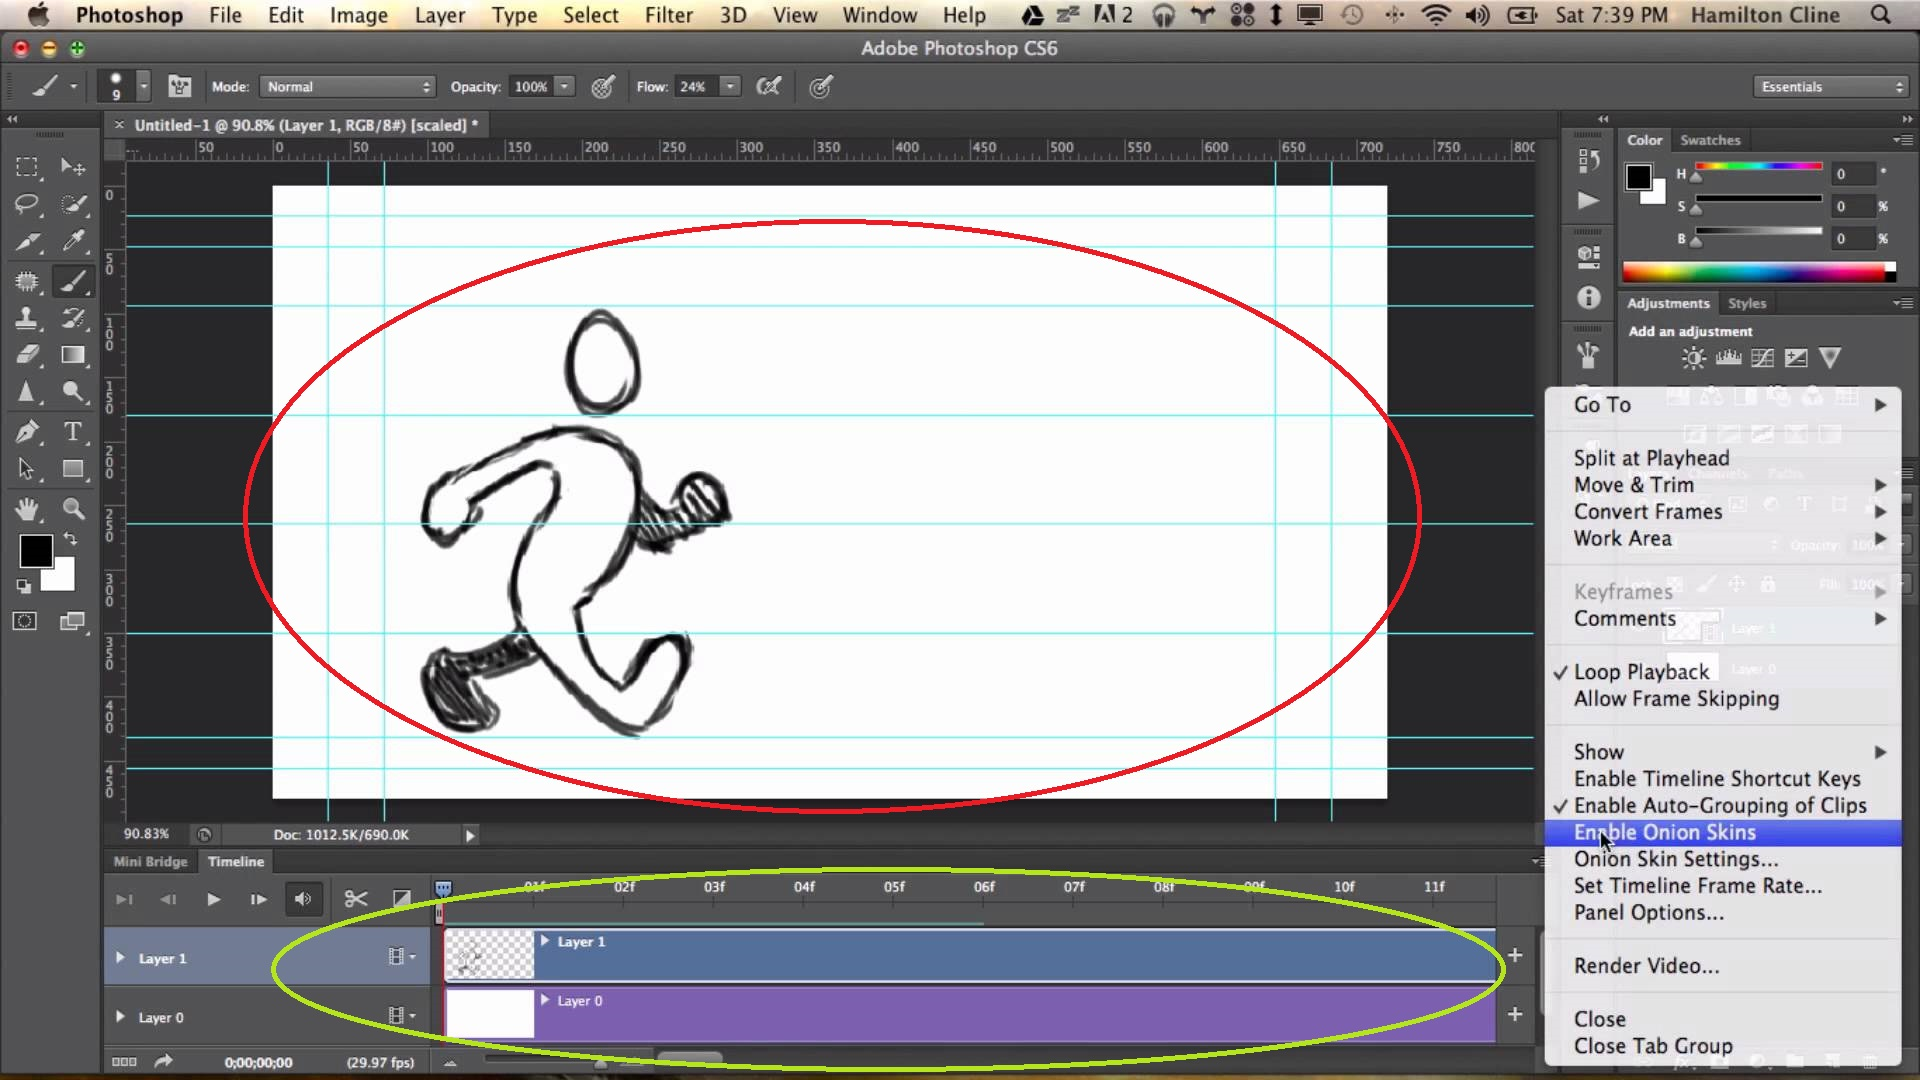
\includegraphics[width=0.95\textwidth]{figs/4-PhotoshopAnimationIDE.png}
\caption{IDE de Photoshop. De color rojo se marca el Canvas y de color verde la animación.}
\label{fig:IDEPhotoshop}
\end{center}
\end{figure}

Una vez definido cuál es el referente en el diseño del entorno de WebMakeUp a seguir, hay que buscar cómo representar las animaciones. Con él, el usuario puede diseñar animaciones sin conocimientos de programación. Este último aspecto limita bastante las opciones de animación que tiene el editor. El incluir aspectos como condiciones, bucles y demás lo haría demasiado complejo.

En el Apartado \ref{sec:modeloSTD} se comenta cuál fue la primera idea de cómo realizar esta representación. En WebMakeUp, tras probarlo con usuarios finales se decide descartar esta representación en favor del uso de blinks (Apartado \ref{sec:modeloBlinks}).

\section{Modelo de diagramas de transición de estados}
\label{sec:modeloSTD}

Para comprender el porqué se decide adoptar el modelo de diagramas de transición de estados (a partir de ahora STD, \emph{State Transition Diagram}) hay que comprender un poco más cómo funcionan las animaciones en Photoshop. En Photoshop las animaciones se producen en base a un evento, el evento temporal. El evento temporal en Photoshop permite cambiar el estado global de la imagen que se está editando, es decir, que existe un evento que hace que se cambie de un estado global a otro.

Pero, ¿qué es el estado global? El estado global en Photoshop lo constituyen, en un instante de tiempo concreto, las capas que están visibles. Las capas en Photoshop equivale a superponer una imagen encima de otra. Habitualmente estas imágenes tienen partes transparentes, que permiten ver la imagen inmediatamente inferior, tal y como se muestra en la Figura \ref{fig:PhotoshopCapas}. Poniendo diferentes capas en diferentes instantes de tiempo se conforman diferentes imágenes y por tanto diferentes estados globales.

\begin{figure}
\begin{center}
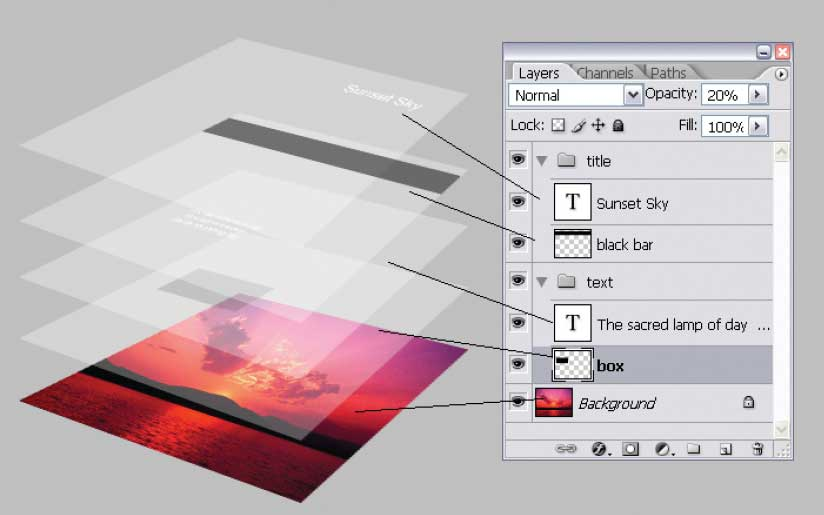
\includegraphics[width=0.35\textwidth]{figs/4-PhotoshopCapas.png}
\caption{Capas de una imagen en Photoshop}
\label{fig:PhotoshopCapas}
\end{center}
\end{figure}


Como se observa en la Figura \ref{fig:PhotoshopTimeline} en cada instante de la línea de tiempo hay diferentes estados globales. En WebMakeUp, se pueden traducir las capas a widgets y los estados de las líneas de tiempo por un STD. Basándose en el artículo  \cite{WhoMovedMyState}, la razón del STD es lógica. Realizar un evento sobre el sitio hace que cambien de estado los widgets, y la suma de los estados de los widgets conforman el estado global (el mismo concepto se utiliza en los sistemas distribuidos y el estado de los nodos \footnote{Gestión de un cluster de IBM PowerVM donde se menciona los 3 posibles estados globales dependiendo del estado de los nodos: \url{http://www-01.ibm.com/support/knowledgecenter/8246-L1T/p7hcgl/cluster.htm}}).

\begin{figure}
\begin{center}
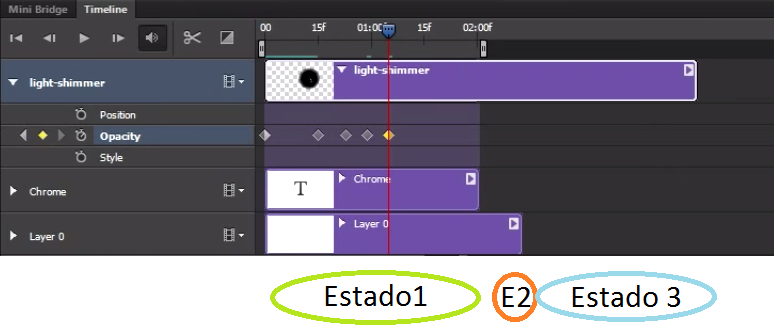
\includegraphics[width=0.75\textwidth]{figs/4-PhotoshopTimeline.png}
\caption{Timeline de Photoshop, donde el estado de las capas a lo largo del tiempo muestra 3 estados globales diferentes.}
\label{fig:PhotoshopTimeline}
\end{center}
\end{figure}

Un STD permite mostrar en un simple vistazo todos los estados posibles de la aplicación y el cómo se llega a esos estados (mediante qué eventos y en qué estado previo).

Pero aún queda por describir qué estados iban a tener los widgets. En un comienzo, como ejemplo de aumentación se toma de referencia una aumentación concreta llamada MyWiki, desarrollada por el grupo de investigación Onekin.

MyWiki es un \emph{userscript} instalable en diferentes navegadores webs (aunque estaba enfocado para Mozilla Firefox). El objetivo de MyWiki es permitir en artículos de Wikipedia\footnote{Sitio web de Wikipedia: \url{http://en.wikipedia.org/}} poder añadir notas y almacenarlas de manera local. En este apartado, se centra únicamente en una funcionalidad muy concreta de cómo está constituida la página web Wikipedia. Tal y como se observa en la Figura \ref{fig:MyWikiAugmentation} existe una nueva pestaña de navegación donde se puede añadir nuestras notas sobre el artículo que se está visitando. Esta pestaña presenta dos estados que pueden resultar interesantes en diferentes tipos de widgets. Estos dos estados son seleccionado y deseleccionado y en uno responde a eventos y en el otro no.

Tomando el ejemplo de MyWiki, además de ser interesante seleccionar y deseleccionar, también hay que tener la opción de ocultar el artículo de XML para mostrar el editor de notas de MyWiki (Figura \ref{fig:MyWikiEditor}).

\begin{figure}
\begin{center}
\subfloat[No augmented Wikipedia]{
	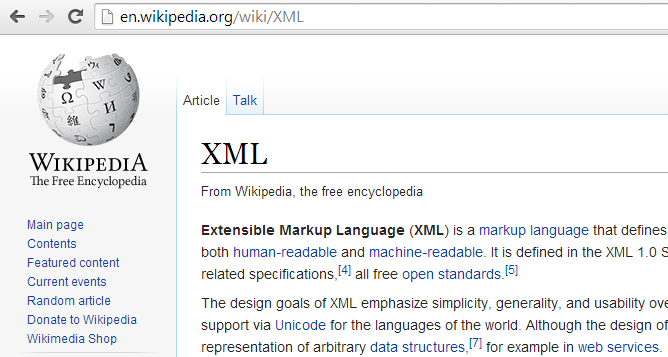
\includegraphics[width=0.47\textwidth]{figs/4-WikipediaXML.png}
}
\subfloat[Augmented with MyWiki]{
	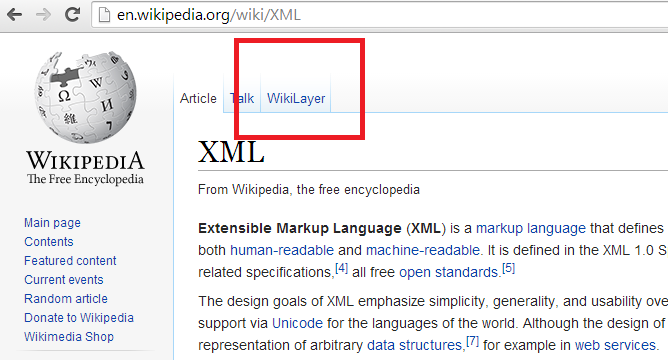
\includegraphics[width=0.47\textwidth]{figs/4-MyWikiTab.png}
}
\caption{A la izquierda artículo de Wikipedia sobre XML. A la derecha el mismo artículo con la aumentación realizada con MyWiki.}
\label{fig:MyWikiAugmentation}
\end{center}
\end{figure}

\begin{figure}
\begin{center}
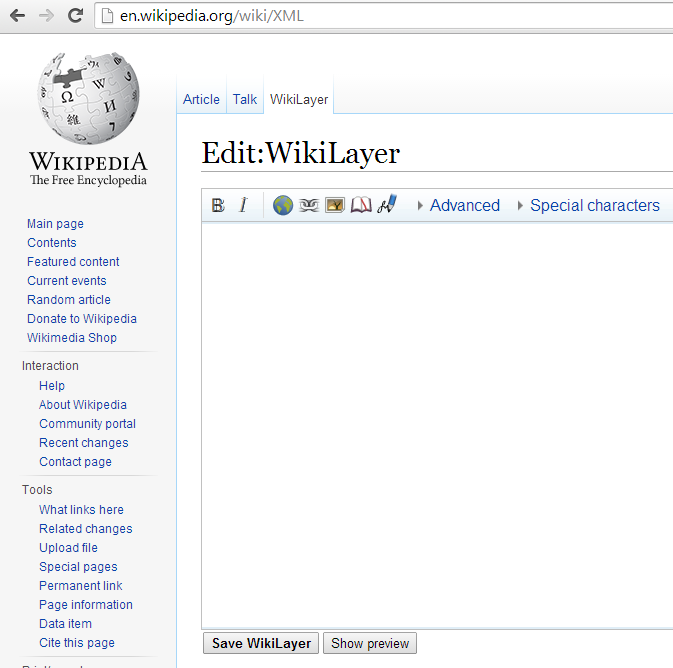
\includegraphics[width=0.45\textwidth]{figs/4-MyWikiEditor.png}
\caption{Editor de MyWiki integrado en Wikipedia.}
\label{fig:MyWikiEditor}
\end{center}
\end{figure}

Los artefactos que se necesitan para describir las interacciones de la aumentación mediante los STD son los siguientes:
\begin{itemize}
\item{Estados: constituido por un nombre (o identificador) y por un listado de los widgets y su estado (selected, deselected o collapsed) en ese estado global.}
\item{Transiciones: constituido por un evento (click, double click, mouseover o mouseout) y en qué widget se produce ese evento para que se dé la transición. Lógicamente, para representar la transición se requiere del identificador del estado origen y del de destino.}
\end{itemize}

Una vez definido los artefactos con los que se va a trabajar solo queda por describir cómo se ha hecho. Para ello hay que hacer un estudio, por un lado de herramientas que permitan describir de manera gráfica, y por otro lado, cómo representar internamente esas interacciones para la futura generación de la extensión con la aumentación \emph{ready to use} (lista para instalar y usar).

Sobre la generación de la extensión se habla en el Capítulo \ref{cha:generador}. En él se menciona el cómo se decide usar una librería llamada ConstraintJS con una sencilla API para trabajar con STDs (ver Anexo \ref{sec:CJS}). En consecuencia, este apartado se centra en cómo se representar de manera gráfica y cómo interactuar entre el diagrama STD y el Canvas.

Para ello, antes de nada, es conveniente estudiar cómo es la primera versión funcional de WebMakeUp. En la Figura \ref{fig:WebMakeUpVer1} se muestran dos paneles, uno izquierdo y otro inferior. El panel izquierdo contiene un repositorio de widgets. Estos se arrastran sobre el Canvas (que es la instancia del sitio web, en este caso Wikipedia). Por otro lado, el panel inferior es donde está el STD. Este está programado íntegramente usando una librería para dibujar diagramas de diferente tipo usando la tecnología Canvas HTML5 (no confundir con el Canvas de WebMakeUp) llamada GoJS. Canvas HTML5 es una nueva característica de HTML5 que permite crear dibujos sobre un lienzo. En el lienzo se dibujan diferentes tipos de objetos (formas geométricas, textos, degradados, imágenes,...) mediante el uso de Javascript.

\begin{figure}
\begin{center}
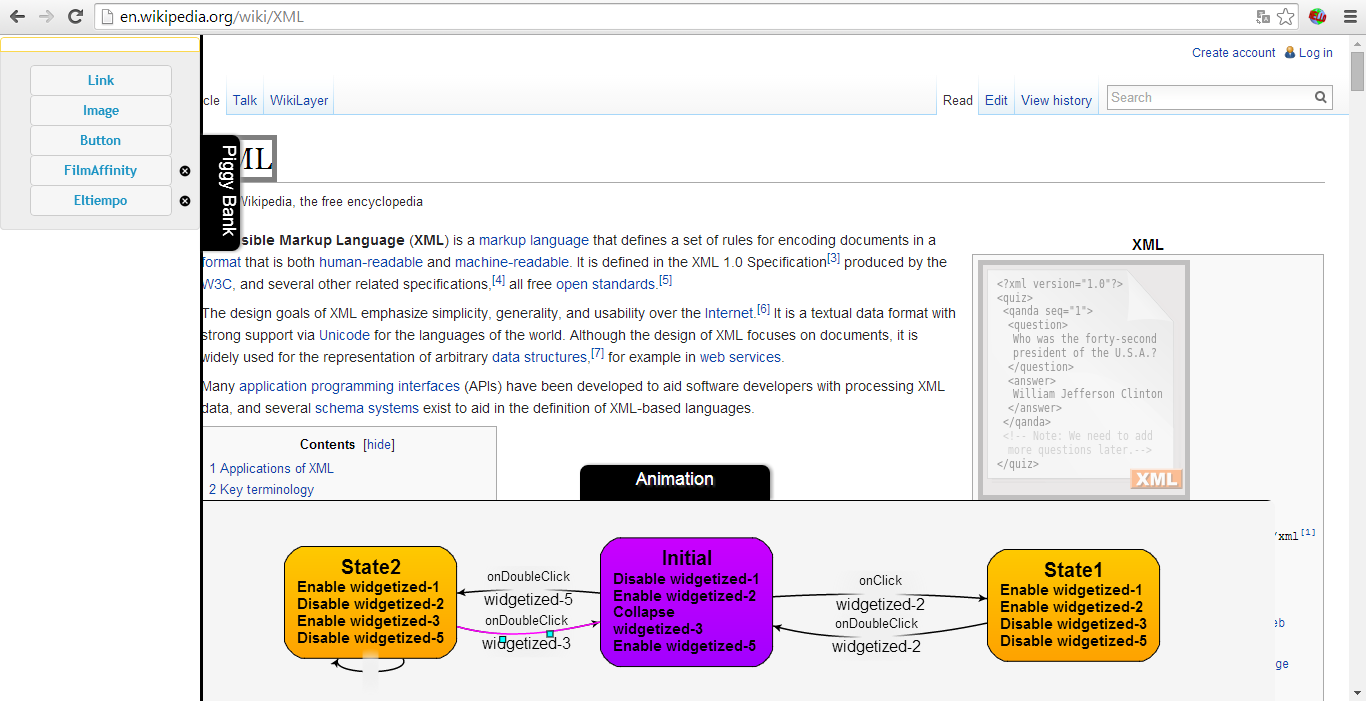
\includegraphics[width=0.95\textwidth]{figs/4-WebMakeUpVer1.png}
\caption{Editor WebMakeUp realizando una aumentación en \url{www.wikipedia.org.}}
\label{fig:WebMakeUpVer1}
\end{center}
\end{figure}

\subsection{GoJS - Librería de gráficas HTML5}
\label{sec:Interacciones-GoJS}

GoJS, tal y como lo describen en su sitio web\footnote{Sitio web de: \url{ http://www.gojs.net/latest/index.html}}, es una librería Javascript para implementar diagramas interactivos en diferentes navegadores actuales. Se basa en nodos, links y grupos para la creación de estos diagramas. Es fácilmente configurable mediante plantillas.

En su sitio ofrecen variedad de ejemplos\footnote{Ejemplo de STD de GoJS: \url{http://www.gojs.net/latest/samples/stateChart.html}} de cómo hacer desde arboles de decisión, EDTs, GANTTs, diagramas de flujo, etc. Se podría decir que es realmente muy configurable, pero la curva de aprendizaje de uso es lenta por dos razones principales:
\begin{itemize}
\item{Al funcionar todo con nodos y links realizar ciertos tipos de diagrama puede ser bastante complejo.}
\item{La API es realmente muy completa, ofrece infinididad de opciones, y la documentación es enorme, pero encontrar cómo se quieren hacer ciertas cosas requiere de búsqueda de alternativas a veces un poco complejas.

Por poner un ejemplo, en los STD de WebMakeUp se requería que el nodo inicial no se pudiera eliminar (ya que al menos se requiere un estado global en una aumentación, el estado inicial). Para realizar esto era necesario definir una capa diferente en el lienzo y crear una plantilla diferente al resto para el nodo inicial. Por tanto, se podría decir mediante este ejemplo que funciona de manera similar a como lo hace Photoshop, con capas. Respecto a las capas no había nada definido en ninguno de los ejemplos, y al ser una librería poco trillada, no era trivial encontrarse con ese método para resolver el problema.}
\end{itemize}

GoJS como se ha comentado, dispone de infinidad de características, y estas son algunas de las que se utilizan en el desarrollo de la interacción basada en STDs:
\begin{itemize}
\item{Es una aplicación desarrollada en Modelo-Vista-Controlador (MVC). El controlador se encarga de gestionar los eventos que se producen en el diagrama (selecciones, borrar nodos o links, etc.). El modelo se encarga de almacenar todos los datos que se generan mientras se trabaja con el editor. La vista se actualiza automáticamente cuando el modelo cambia, lo que favorece mucho el desarrollo ya que los cambios se reflejan automáticamente.}
\item{Las plantillas permiten definir cómo se van a presentar los datos, pero además reflejan qué datos van a estar en el modelo y cómo se va a hacer el \emph{matching} (la concordancia) entre los datos. Por ejemplo, se puede definir que en la vista se muestren los nombres de los widgets presentes en un estado del STD, pero internamente sólo se almacena el identificador.}
\item{GoJS al ser también un editor, en este caso de gráficas en HTML5, permite exportar e importar el modelo de manera sencilla en un objeto JSON, que es como se representan los objetos en Javascript. En el caso de los STDs el JSON que se obtiene es del estilo del que se muestra en la Figura \ref{fig:GoJSModelJSON}}.
\item{De igual manera, como la mayoría de editores dispone de características de edición que son difíciles de implementar, UNDO y REDO (deshacer y rehacer). En la Figura \ref{fig:GoJSTransaction} se muestra cómo GoJS funciona con transacciones, igual que las bases de datos convencionales. Las transacciones se van almacenando y gracias a ello se puede hacer UNDO y REDO.}
\end{itemize}

\begin{figure}
\begin{center}
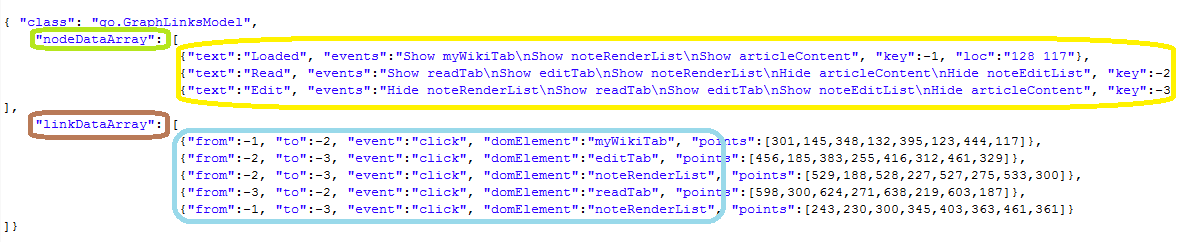
\includegraphics[width=0.95\textwidth]{figs/4-GoJSModelJSON.png}
\caption[Modelo generado por GoJS con información de los estados y transiciones del STD.]{Modelo generado por GoJS con información de los estados y transiciones del STD. De color verde y marrón la declaración de la lista de nodos y transiciones. De color amarillo, la información de los nodos y de azul la de las transiciones.}
\label{fig:GoJSModelJSON}
\end{center}
\end{figure}

\begin{figure}
\begin{center}
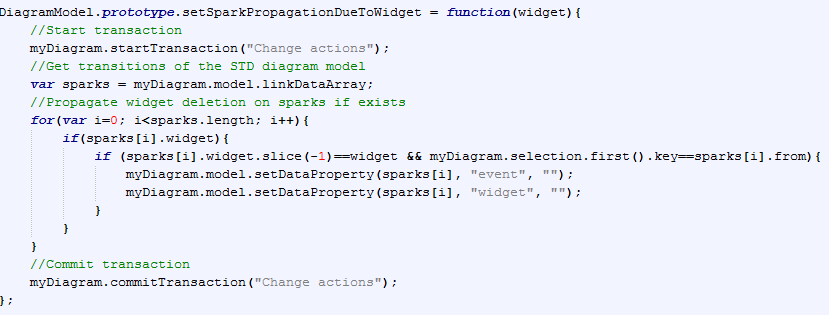
\includegraphics[width=0.95\textwidth]{figs/4-GoJSTransaction.png}
\caption{Funcionamiento de transacciones en el modelo de datos de GoJS.}
\label{fig:GoJSTransaction}
\end{center}
\end{figure}

Estas características permiten que se puedan comunicar mediante una API (basada en restricciones con ConstraintJS) el Canvas y el STD.

Sobre ConstraintJS se habla en el Anexo \ref{sec:CJS}, aunque cabe destacar que es una librería que permite trabajar con restricciones y en base a cambios en esas restricciones ejecutar manejadores (handlers, funciones Javascript) de manera automatizada. 

Por ejemplo, el cambiar el nodo seleccionado en el STD implicaba cambiar de estado de los widgets en el Canvas, tal y como se puede observar en la Figura \ref{fig:WebMakeUpV1NodeSelection}.

\begin{figure}
\begin{center}
\subfloat[Selected state A]{
	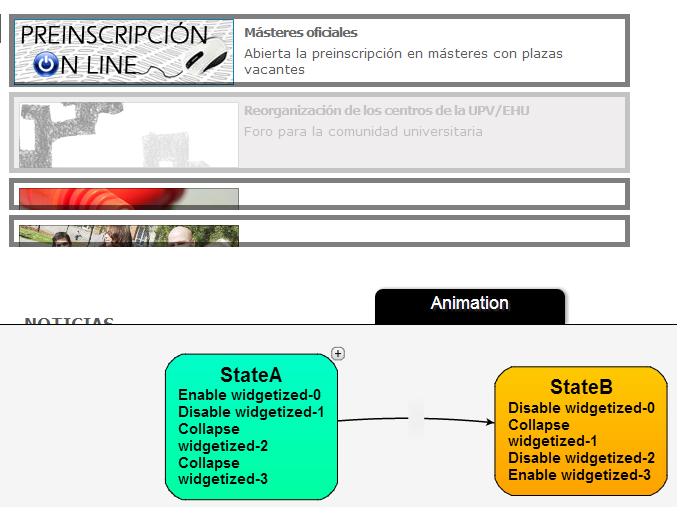
\includegraphics[width=0.47\textwidth]{figs/4-WebMakeUpV1SelectedA.png}
}
\subfloat[Selected state B]{
	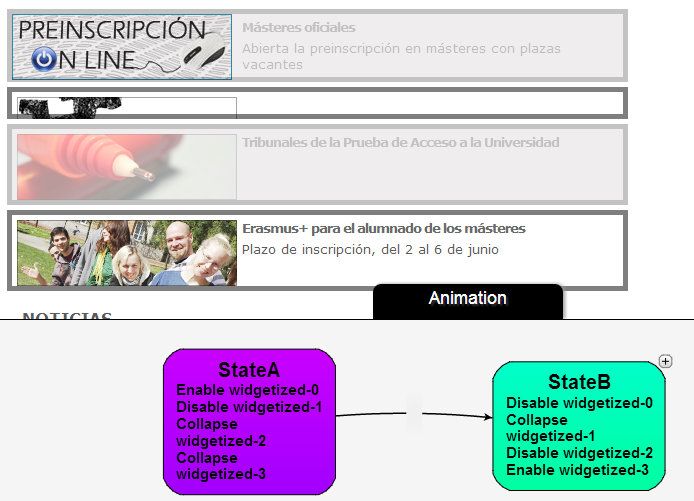
\includegraphics[width=0.47\textwidth]{figs/4-WebMakeUpV1SelectedB.png}
}
\caption{Cambio de estado de los widgets al seleccionar diferentes estados del STD.}
\label{fig:WebMakeUpV1NodeSelection}
\end{center}
\end{figure}

\section{Modelo de blinks}
\label{sec:modeloBlinks}

Tras la realización de un estudio con usuarios finales que no se realizó dentro del PFG, se detectaron muchos aspectos a mejorar. En lo que concierne al PFG, cabe destacar que el diagrama de transición de estados (Apartado \ref{sec:modeloSTD}) era complejo para la mayoría de usuarios por las siguientes razones:
\begin{itemize}
\item{El concepto de estado global es complejo. No se visualiza de manera sencilla la aumentación y lo que se quería aumentar.}
\item{La representación fuera del Canvas resulta confusa. El tener que conocer el nombre de cada uno de los widgets para poder comprender el STD y por tanto las transiciones, hace tediosa la programación de las interacciones.}
\item{El estado deselect no es muy utilizado. Se considera que un estado mostrado y otro ocultado son suficientes.}
\item{No es escalable para los propósitos de los usuarios. Por ejemplo para definir botones que ocultan o mostraban widgets concretos haciendo clic sobre ellos (algo bastante utilizado). Si se definen 3 de este tipo equivale a tener que realizar una máquina de 9 estados. \[x=n^2 / n=numeroDeBotones\] En la Figura \ref{fig:EscalabilidadInteracciones} se refleja la sencillez de los blinks frente a la complejidad de los STD en este caso.}
\end{itemize}

\begin{figure}
\begin{center}
\subfloat[Modelo basado en STD]{
	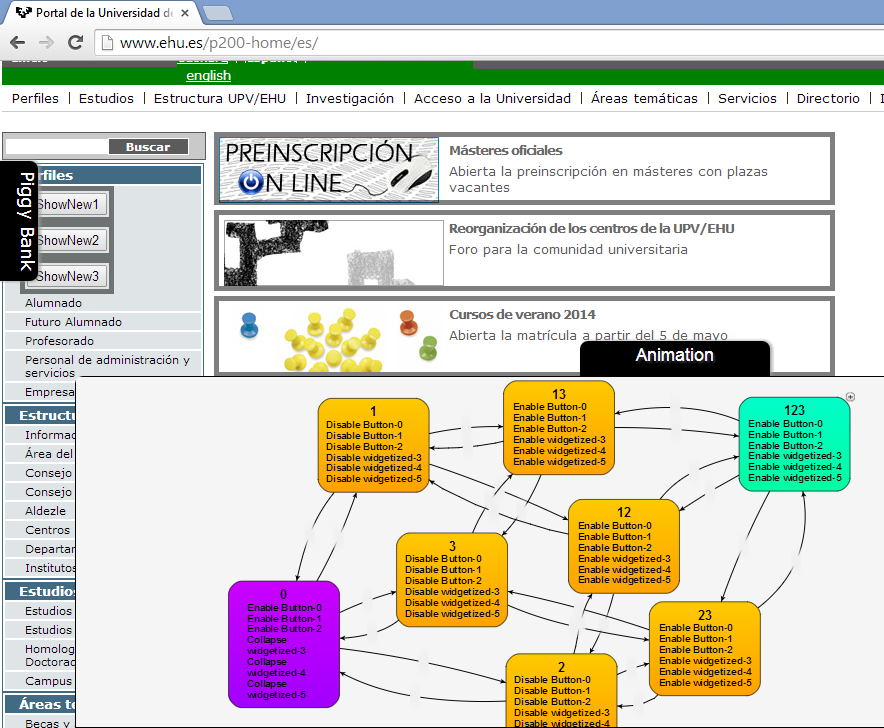
\includegraphics[width=0.45\textwidth]{figs/4-ScalabilitySTD.png}
}
\subfloat[Modelo basado en Blinks]{
	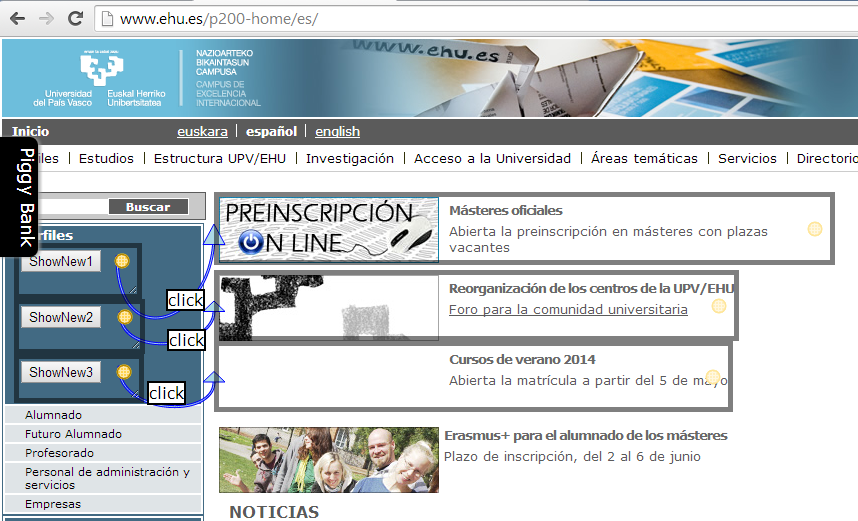
\includegraphics[width=0.45\textwidth]{figs/4-ScalabilityBlink.png}
}
\caption{Comparativa de escalabilidad entre el modelo basado en STD y el modelo basado en blinks.}
\label{fig:EscalabilidadInteracciones}
\end{center}
\end{figure}

Todo este feedback obtenido por parte de los usuarios ha servido para idear otra técnica que es más acorde, solventando los inconvenientes y tratando de aprovechar en la mayor medida posible el trabajo ya previamente realizado.

Esta técnica se basa en un concepto llamado blink, donde los widgets pestañean, es decir, están mostrándose u ocultándose. Ahora no existe un estado global conocido para el usuario, él simplemente tiene que indicar en qué widget se produce el evento para que el widget al que apunta pestañee y cambie su estado de mostrado (\emph{enabled}) a oculto (\emph{collapsed}) o viceversa. Esto se realiza en base a links tal y cómo se observa en la Figura \ref{fig:BlinkLink}.

\begin{figure}
\begin{center}
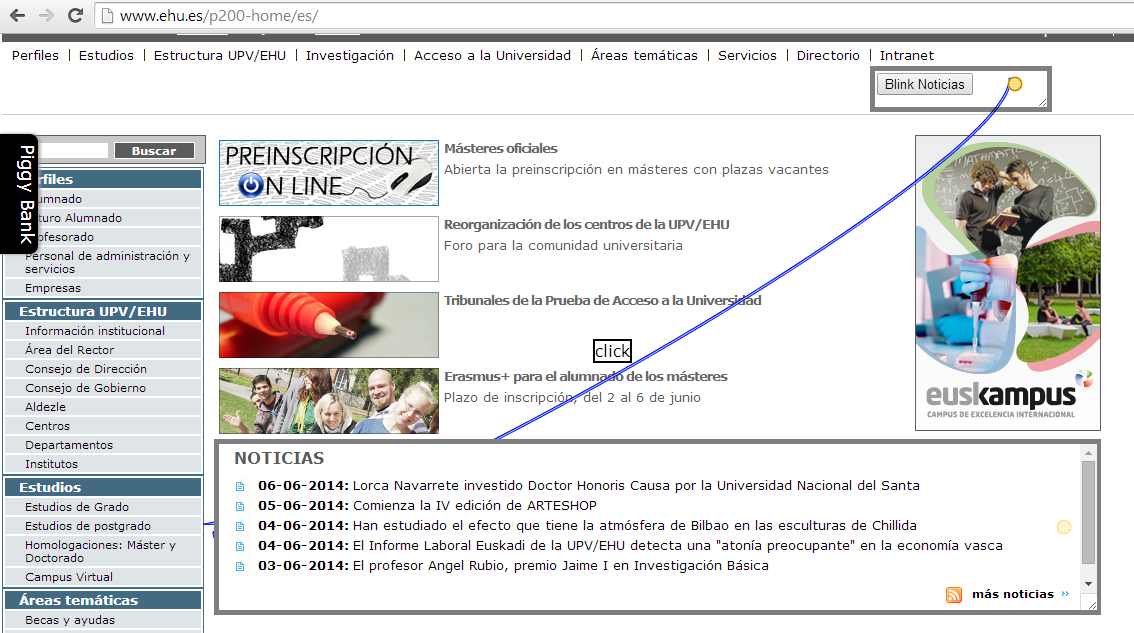
\includegraphics[width=0.55\textwidth]{figs/4-BlinkLink.png}
\caption[WebMakeUp con interacciones mediante el modelo de blinks.]{Editor WebMakeUp con interacciones mediante blinks, con dos widgets conectados mediante un link. El superior es el controlador y el inferior el observador.}
\label{fig:BlinkLink}
\end{center}
\end{figure}

Mediante la técnica de blink por tanto se tienen dos widgets que entran en juego. A uno se le llama el widget observador, que es el que observa si se ha producido un evento en el widget controlador. Si en el widget controlador se produce un evento el observador realiza un blink (es decir, cambia su estado de enable a collapse, o viceversa).

Para ello hay que tener en cuenta un nuevo aspecto, el de eventos opuestos. El evento opuesto es el evento que se tiene que producir para que el observador regrese al estado inicial. En WebMakeUp se definen cuatro eventos: \emph{click}, \emph{double click}, \emph{mouseover} y \emph{mouseout}. Hay que tener en cuenta que mouseover y mouseout están relacionados, es decir, que cuando se pone el cursor sobre un widget se hace un mouseover, y cuando se mueve fuera del widget, se produce un mouseout. Teniendo en cuenta esto, se definen tres eventos y sus opuestos:
\begin{itemize}
\item{Click y su opuesto, que es el propio click. En consecuencia, en el ejemplo de la Figura \ref{fig:BlinkLink}, cada vez que se haga clic en el widget controlador, el observador irá alternandose entre enabled y collapsed.}
\item{DoubleClick y su opuesto, el propio doubleClick.}
\item{Mouseover y su opuesto, mouseout. A este par en WebMakeUp se le llama MouseEnter.}
\end{itemize}

La definición del metamodelo de los blink se puede representar de la manera que se observa en la Figura \ref{fig:BlinkMetamodel}. En el metamodelo hay dos clases, la de widgets y la de blinks. 

La clase \textbf{Widget} representa toda la información del widget. En este caso únicamente se necesita conocer su identificador y el estado inicial. El identificador sirve para crear las relaciones entre widgets. El estado inicial, indica cuál es el estado por defecto del widget. Esto es importante, dado que gracias a definir si un widget inicia en enabled o collapsed, se consiguen generar diferentes tipos de patrones. Esto se explica detalladamente en el Apartado \ref{sec:PatronesBlinks}.

La clase \textbf{Blink} representa la relación de dos widgets (un controlador y un observador). A su vez, hay que tener en cuenta cuál de los tres eventos (DOMEventType) tiene que esperar el observador.

\begin{figure}
\begin{center}
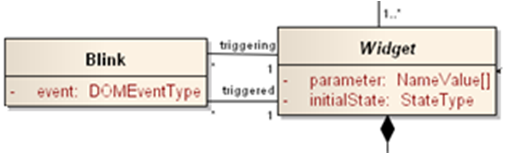
\includegraphics[width=0.45\textwidth]{figs/4-BlinkMetamodel.png}
\caption{Parte del metamodelo de WebMakeUp que representa los blinks.}
\label{fig:BlinkMetamodel}
\end{center}
\end{figure}

Cabe destacar que en este PFG, a diferencia del modelo basado en STD, donde sí se trabajó sobre la presentación al usuario final, en los blinks no fue así. La librería utilizada para dibujar fue WireIt \footnote{Sitio oficial de WireIt: \url{http://neyric.github.com/wireit}} con pequeñas modificaciones adaptándolas a las necesidades de WebMakeUp. Lo que sí se trabajó fue la generación de la extensión de Google Chrome a partir de este nuevo modelo basado en blinks. Esto está desarrollado en el Capítulo \ref{cha:generador}.

\subsection{Patrones de blinks}
\label{sec:PatronesBlinks}

A raíz del paradigma basado en blinks, se pueden definir diferentes tipos de patrones de diseño. Estos patrones de diseño, permiten ayudar a la hora de diseñar interacciones que se pueden dar habitualmente en las aumentaciones web. El usuario simplemente tiene que elegir qué widgets interaccionan y qué patrón de los propuestos siguen. Esto lo que realizará será de manera automatizada añadir las flechas correspondientes que hacen que se cumpla con el patrón deseado. 

Los patrones de diseño juegan con dos aspectos clave en el modelo basado en Blinks. Por un lado, el estado inicial de los widgets. Predefinir adecuadamente el estado inicial de un widget (mostrándose u ocultándose), permite generar diferentes patrones. Por otro lado, el número de widgets participantes en la interacción. Aunque las interacciones se hagan con un observador y un controlador, la unión de varias interacciones en una misma aumentación permite obtener diferentes patrones de diseño.

\begin{figure}
\begin{center}
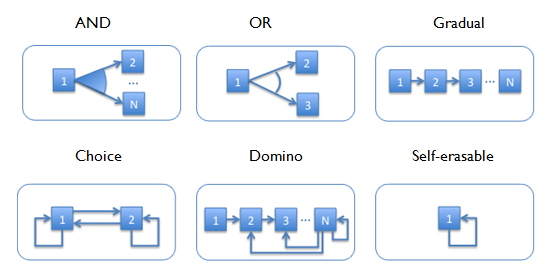
\includegraphics[width=0.95\textwidth]{figs/4-PatronesBlinks.png}
\caption{Patrones de diseño basado en blinks predefinidos en WebMakeUp.}
\label{fig:PatronesBlink}
\end{center}
\end{figure}

En la Figura \ref{fig:PatronesBlink} se observan los diferentes patrones que ahora se comentan en detalle:

\begin{itemize}
\item{Patrón AND: este patrón permite que al interactuar con un widget controlador se muestren/oculten varios widgets de manera simultánea. Para ello el patrón prepara a todos los widgets con el mismo estado inicial, con tal de que estos a medida que se produzcan los blinks, sigan compartiendo el mismo estado (todos mostrándose o todos ocultos).
 
Es útil cuando se quiere mostrar u ocultar varios widgets simultáneamente.}
\item{Patrón OR: este patrón tiene sentido con 3 widgets, un controlador y 2 observadores. En este caso en cada blink, uno de los observadores se mostrará (el que estuviera oculto) y el otro se ocultará (el que estuviera mostrándose). El funcionamiento es igual que el del AND, con la única diferencia de que el estado inicial no es el mismo en todos los widgets.

Es útil cuando se quiere alternar el contenido que se está mostrando.}
\item{Patrón Gradual: el funcionamiento consiste en indicar varios widgets, donde cada uno al interactuar con él muestra más contenido.

Es útil cuando existe contenido con jerarquía o de árbol, es decir, cuando hay contenido que depende de otro contenido para tener utilidad en la web.}
\item{Patrón Choice: permite alternar entre dos widgets, si se muestra uno el otro estará oculto y viceversa. El intercambio se produce realizando una interacción sobre él mismo.

Esto es útil cuando se quiere ir alternando entre diferente contenido sin necesidad de otro widget.}
\item{Patrón Domino: el funcionamiento es similar al de un dominó, donde al interaccionar con un widget muestra el siguiente y así sucesivamente. Cuando se interacciona con el último este oculta todos los anteriores (exceptuando el primero, para que pueda volver a producirse el efecto dominó).

Esto es útil en información de tipo jerárquica.}
\item{Patrón Self-erasable: al interactuar con él se oculta, no volviendo a mostrarse nunca más hasta que se vuelva a visitar el sitio web.

Esto es útil en caso de información que se quiere leer una vez y no más. Un ejemplo ya implementado en los sitios web por ley actualmente, son los widgets con la advertencia de uso Cookies de terceros.}
\end{itemize}

El uso de estos patrones permite generar dinamismo a los sitios web de manera muy ágil y sencilla.

La razón de utilizarlo de esa manera surge de los SmartArt de Microsoft PowerPoint. Los SmartArt son elementos gráficos que permiten generar diferentes patrones de disposición de los datos, de forma piramidal, jerárquica, cíclica, etc.

En SmartArt, simplemente hay que seleccionar qué datos se toman en cuenta y se elige un patrón. De manera automática, genera un gráfico con la representación de esos datos. En la Figura \ref{fig:SmartArt} se muestra cómo la estructura de datos se convierte en un gráfico que representa mejor el círculo PDCA\footnote{Ciclo de mejora continua o círculo de Deming: \url{http://en.wikipedia.org/wiki/PDCA}}.

En WebMakeUp el funcionamiento es igual. Se seleccionan los widgets participantes y el patrón que van a seguir. De manera automática se generan los diferentes links entre los widgets participantes cumpliendo con ese patrón.

\begin{figure}
\begin{center}
\subfloat[Estructura por defecto]{
	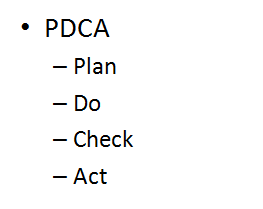
\includegraphics[width=0.45\textwidth]{figs/4-SmartArtDefault.png}
}
\subfloat[Gráfico SmartArt]{
	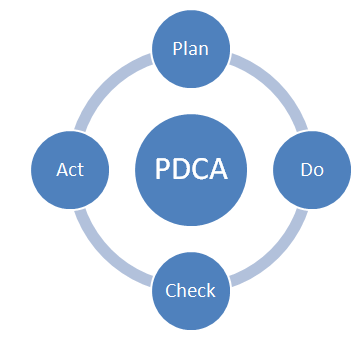
\includegraphics[width=0.45\textwidth]{figs/4-SmartArtGraph.png}
}
\caption{Representación por defecto y gráfica del ciclo PDCA mediante SmartArt de PowerPoint.}
\label{fig:SmartArt}
\end{center}
\end{figure}

Estos patrones no se desarrollaron en este PFG, pero sirven para validar el generador de extensiones. Estos patrones tienen que ser capaces de funcionar en tiempo de ejecución de la aumentación (Apartado \ref{sec:ValidacionGenerador}).

Para finalizar con este capítulo, cabe destacar que al estar aún en pleno desarrollo WebMakeUp, todavía quedaría por realizar una prueba con usuarios reales para ver cómo se adaptarían a estos nuevos cambios. Aunque tal y como se ha ido observando en el trabajo con los blinks la realización de aumentaciones con interacciones es más rápida, y se confía en la buena aceptación del público en general.